\documentclass{article}
\usepackage{fullpage} % sets more standardized margins
\usepackage{graphicx} % some graphics functions I use 
\usepackage{abstract} % abstract function
\usepackage{amsmath}  % math stuff
\usepackage{float}
\usepackage{mathrsfs}
\usepackage[utf8]{inputenc}
\usepackage[document]{ragged2e}
\usepackage{subfiles}
\usepackage{caption}
\usepackage{subcaption}
\usepackage{verbatim}
\usepackage[toc,page]{appendix}
\usepackage{pdfpages}

\renewcommand{\absnamepos}{flushleft} % left justifies abstract
\setlength{\absleftindent}{0pt}
\setlength{\absrightindent}{0pt}



% % %
% Set up IEEE style paragraphing
% % %
\setlength{\parskip}{1em} % The \par command now skips a line between paragraphs, eliminates warnings from using the \par or \\ commands
\setlength{\parindent}{0em} % Left justifies paragraphs after a \par command 


\begin{document}

\pagenumbering{gobble} % Turn off page numbering for titles and tables


\begin{titlepage}
    \begin{center}
        
         \vspace*{1.5cm}
        
    %Berkay suggested this title in the meeting
         \textbf{{\Huge Final Report }}
        
         \vspace{0.5cm}
         \textbf{Optical Link}
        
          \vspace{.5cm}
        
         \textbf{{\Large Joseph Arsenault \\ Ryan Dufour \\ Phil Robb \newline}}
         \textbf{Team 7}
    \vspace{.4cm}
  
    	
    \vspace{1cm}
    
        
        
        \begin{abstract}
        
        
        %I re-worded it here, check it over to make sure it sounds not so choppy and details what is needed
        
        \noindent 
 		The design, simulation and test of an infrared optical link transmitter and receiver is described. The optical link is required to transmit and recieve at a distance of at least 50 ft. The transmitter should send a signal of 20 kHz $\pm$5\%. The signal is required to have a duty-cycle of 50\% $\pm$5\%. The LED driver current is required to be less than 200 mA. The final circuit transmitted 77 ft with a 20.1 kHz signal with a 50.1\% duty-cycle. The LED driver current was 150 mA.  The transmitter consumed 540 mW of power. The receiver consumed. 14.4 mW of power.  Figure \ref{fig:screen-shot-2017-12-11-at-3} below is the block diagram of the optical link project.
 		
 		\begin{figure}[H]
 			\centering
 			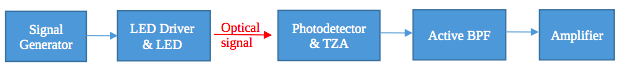
\includegraphics[width=0.7\linewidth]{blockdiagram}
 			\caption[Optical link block diagram]{Optical link block diagram \cite{b1}}
 			\label{fig:screen-shot-2017-12-11-at-3}
 		\end{figure}
 		
        
        
        
        %An LF347 wide bandwidth quad JFET input operational amplifier integrated circuit, MFBP filter, with rail voltages of $\pm$12V, was used to amplify the output signal from a transimpedance amplifier. This is used as a module for an optical uplink circuit. The filter is required to have a center frequency of 20kHz, a 3dB bandwidth between 1.5kHz and 5kHz, a gain of greater than 60dB, and rail supplies of $\pm$12V. A sinusoidal waveform with an amplitude of 100mV and frequency of 20kHz was used for the input to the MFBP filter. The output voltage operated with a gain of 71.4dB, with a bandwidth at 3dB of 2.11kHz and a center frequency of 20.2kHz. 
        \end{abstract}
        
        
        \vspace{02.5cm}
        \textbf{
        Electrical and Computer Engineering\\
        University of Maine\\
        ECE - 342\\\ \today}
    \vspace{.5cm}
    
    \end{center}
\end{titlepage}


\clearpage

\pagenumbering{arabic} % Turn on page numbering



\section{Introduction}


Table \ref{tab:opticallink} shows the device specifications and measured performance of the Optical Link project.

\begin{table}[H]
	\centering
	\caption{Performance summary of optical link project}
	\label{tab:opticallink}
	\begin{tabular}{|l|l|l|l|}
		\hline
		\multicolumn{1}{|c|}{\textbf{Parameter}}                                     & \multicolumn{1}{c|}{\textbf{Specified Value}} & \multicolumn{1}{c|}{\textbf{Measured Value}} & \multicolumn{1}{c|}{\textbf{Reference}} \\ \hline
		Transmission distance (in feet)                                              & $>$ 50'                                       & 77'                                          &         Final                              \\ \hline
		Signal Frequency                                                             & 20 kHz $\pm$ 5\%                              & 20.1 kHz                                     &    Appendix E Page 11                                     \\ \hline
		Duty cycle of signal                                                         & 50\% $\pm$ 5\%                                & 50.1 \%                                      &     Appendix E Page 11                                    \\ \hline
		LED Peak drive current                                                       & $<$200mA                                      & 150 mA                                       &   Appendix E Page 11                                      \\ \hline
		Transmitter Power Consumption                                                & -                                             &  540 mW                                            &    Final                                     \\ \hline
		Receiver Power Consumption                                                   & -                                             &    14.4 mW                                          &       Final                                  \\ \hline
		Frequency sensitivity to capacitor tolerance in ring oscillator (simulation) & -                                             &              -                                &   Appendix D Page 14                                      \\ \hline
	\end{tabular}
\end{table}


Table \ref{tab:simcompare} shows the comparison from simulated values and those measured in the final device.
\begin{table}[H]
	\centering
	\caption{Simulated and measured comparison]}
	\label{tab:simcompare}
	\begin{tabular}{|l|l|l|l|}
		\hline
		\multicolumn{1}{|c|}{\textbf{Parameter}} & \multicolumn{1}{c|}{\textbf{Specified Value}} & \multicolumn{1}{c|}{\textbf{Measured Value}} & \multicolumn{1}{c|}{\textbf{Simulated Value}} \\ \hline
		Signal Frequency                         & 20 kHz $\pm$ 5\%                              & 20.1 kHz                                     & 20 kHz                                        \\ \hline
		Duty cycle of signal                     & 50\% $\pm$ 5\%                                & 50.1 \%                                      & 48 \%                                         \\ \hline
		LED Peak drive current                   & $<$200mA                                      & 150 mA                                       & 200 mA                                        \\ \hline
	\end{tabular}
\end{table}

The circuit operated as expected and within specifications. A rather large modification that was required was the removal of the final voltage amplifier, Task 5. This circuit ended up introducing far too much noise into the final design and resulted in more harmonic distortion. The final circuit met specification without the addition of the voltage amplifier. The final circuit did not need the 200 mA simulated. This is because the real IR LED should be driven with less than 200 mA of current. The circuit was simulated with 200 mA as a way of ensuring, upon circuit implementation, that the LED had enough current to operate. The final circuit acheived 77 ft transmission with a power consumption of 540 mW for the transmitter and 14.4 mW for the reciever.

All prerequisite design documentation are attached as appendices as well as the final schematic and project pictures.  
 
    
    \newpage
\clearpage

\appendix

\begin{thebibliography}{00}



\bibitem{b1} N.W. Emanatoglu "Lab $\#1$; photodetector and transimpedence amplifier," University of Maine, Orono, ME, 2017.
\newline

\newpage


\end{thebibliography}

\begin{appendices}
	
	
\section{Optical Link schematic and pictures.}
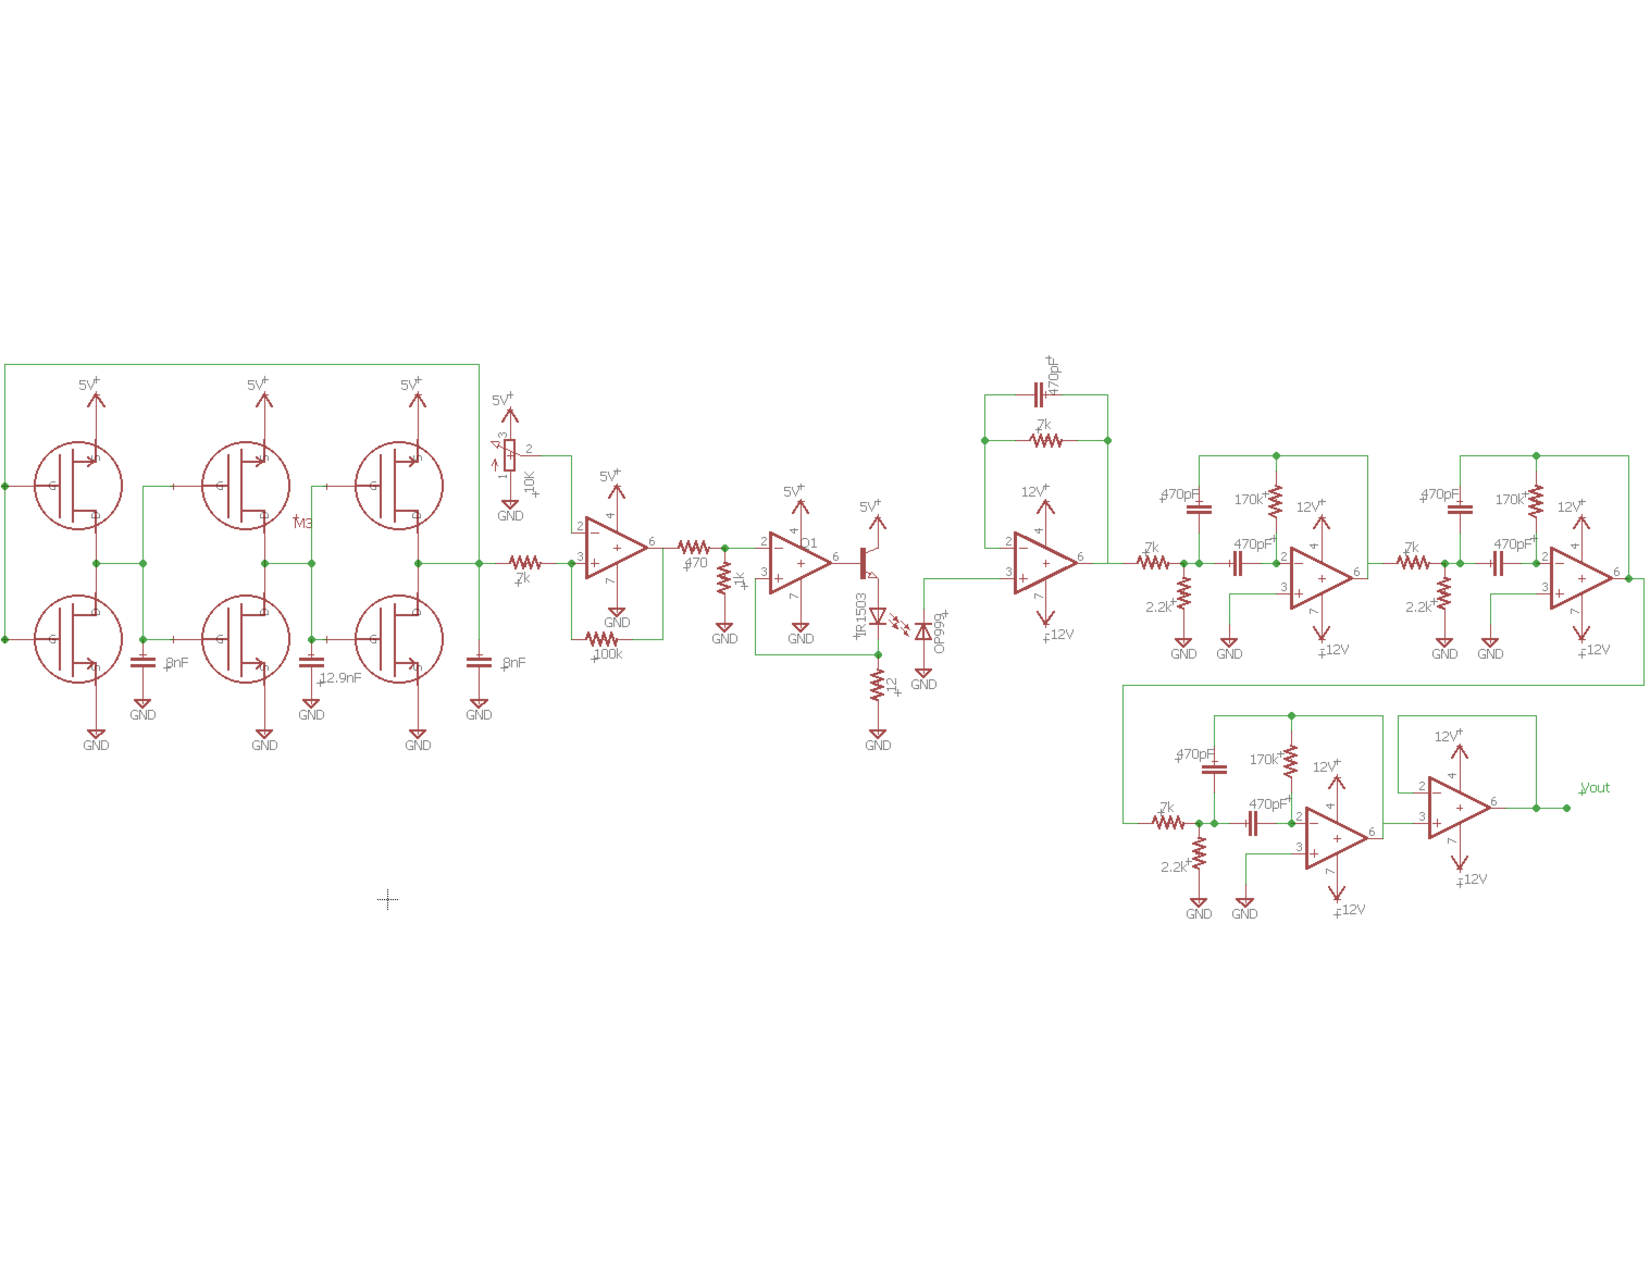
\includepdf[pages=-]{finalfinal.pdf}


\section{Transimpedence Amplifier}
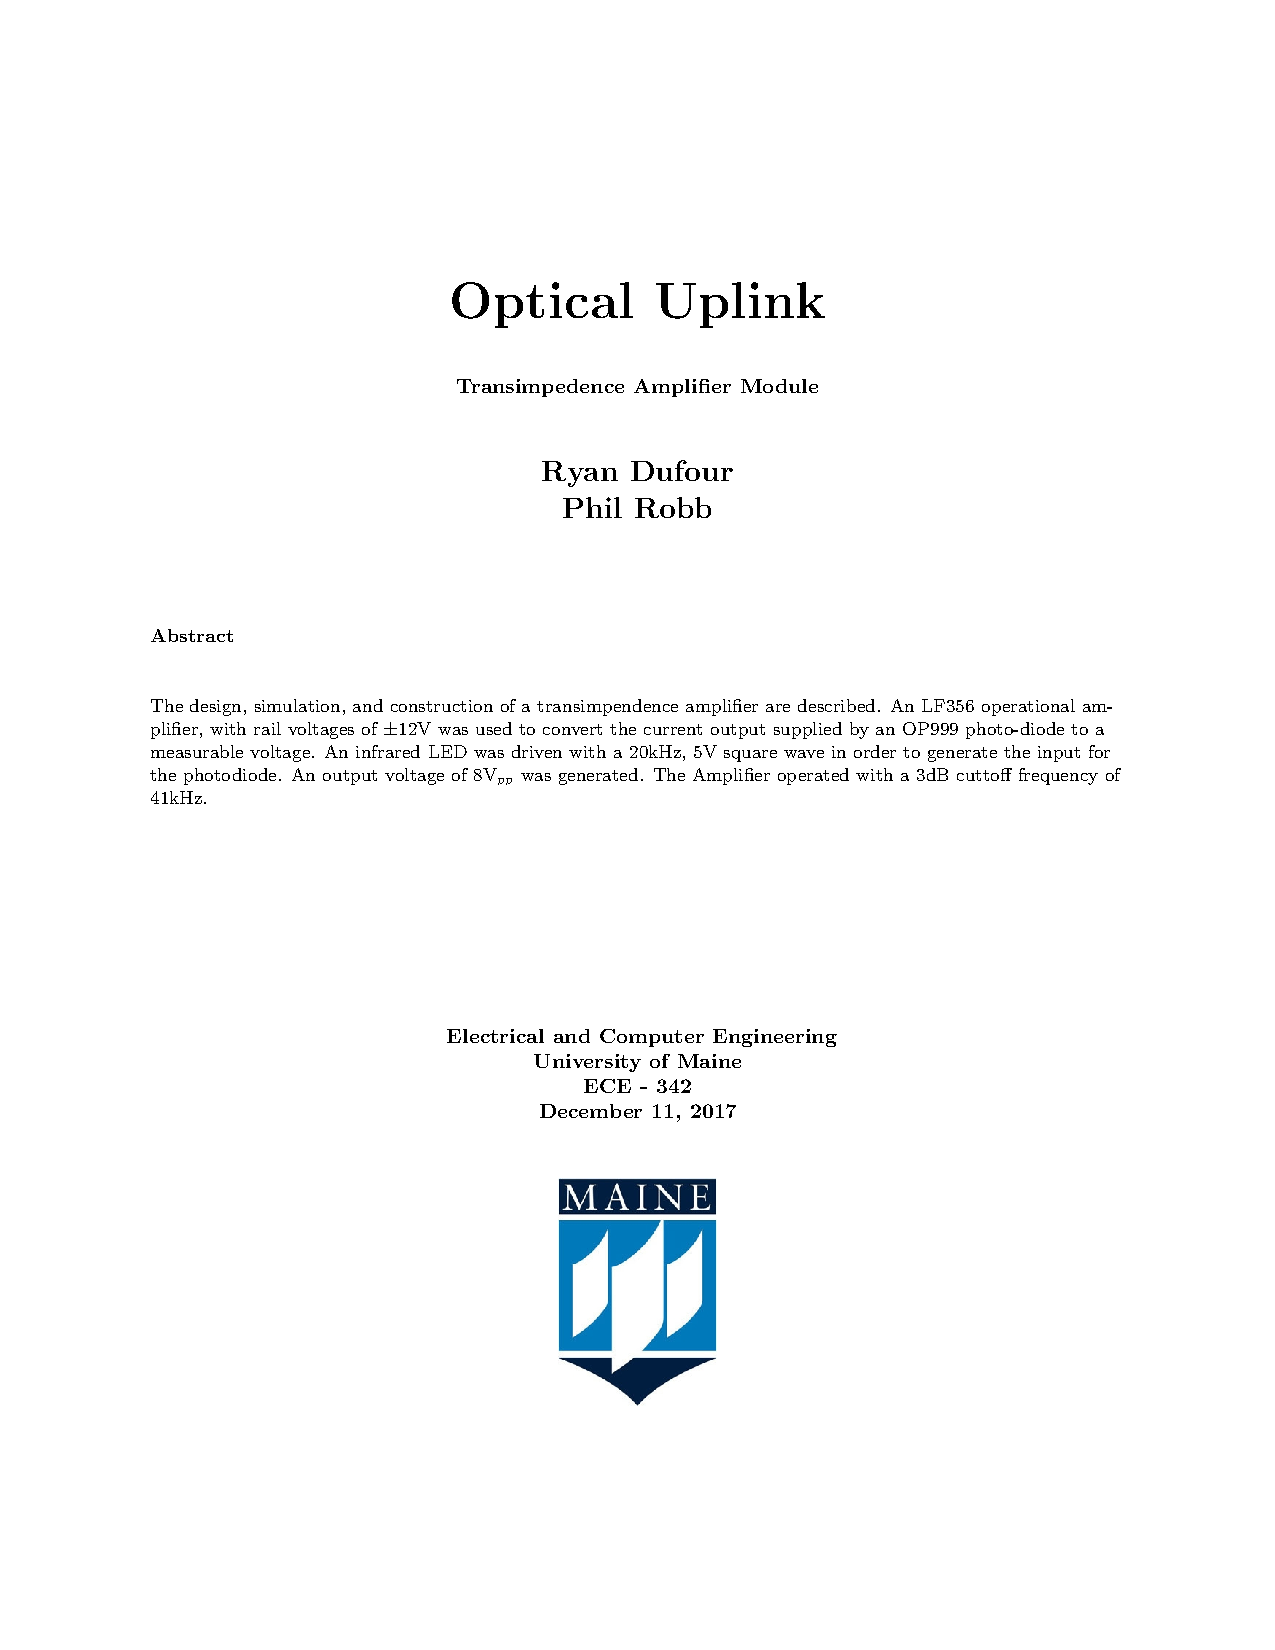
\includepdf[pages=-]{Lab_1.pdf}	

\section{Multifeedback Bandpass Filter}
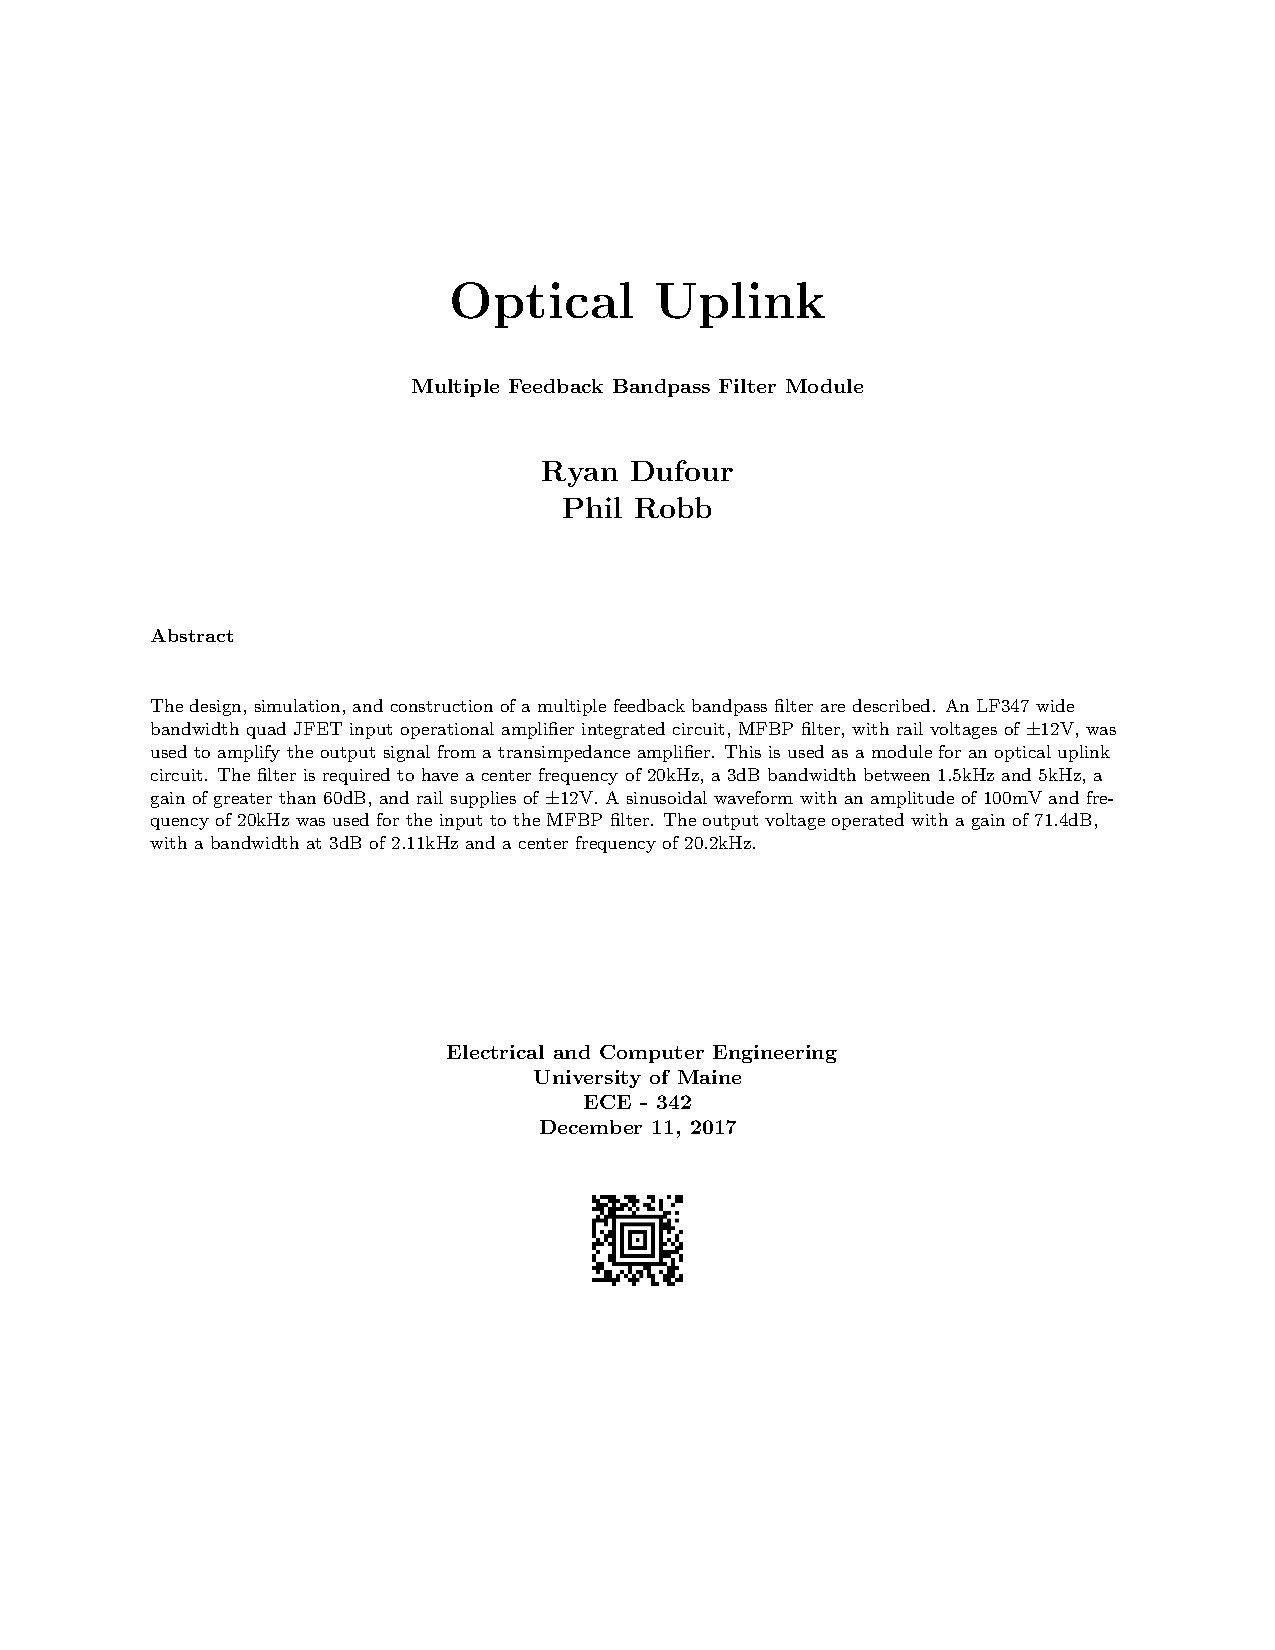
\includepdf[pages={-}]{Lab_2.pdf}	

\section{MOSFET Based Logic Gates and Digital Oscillator}
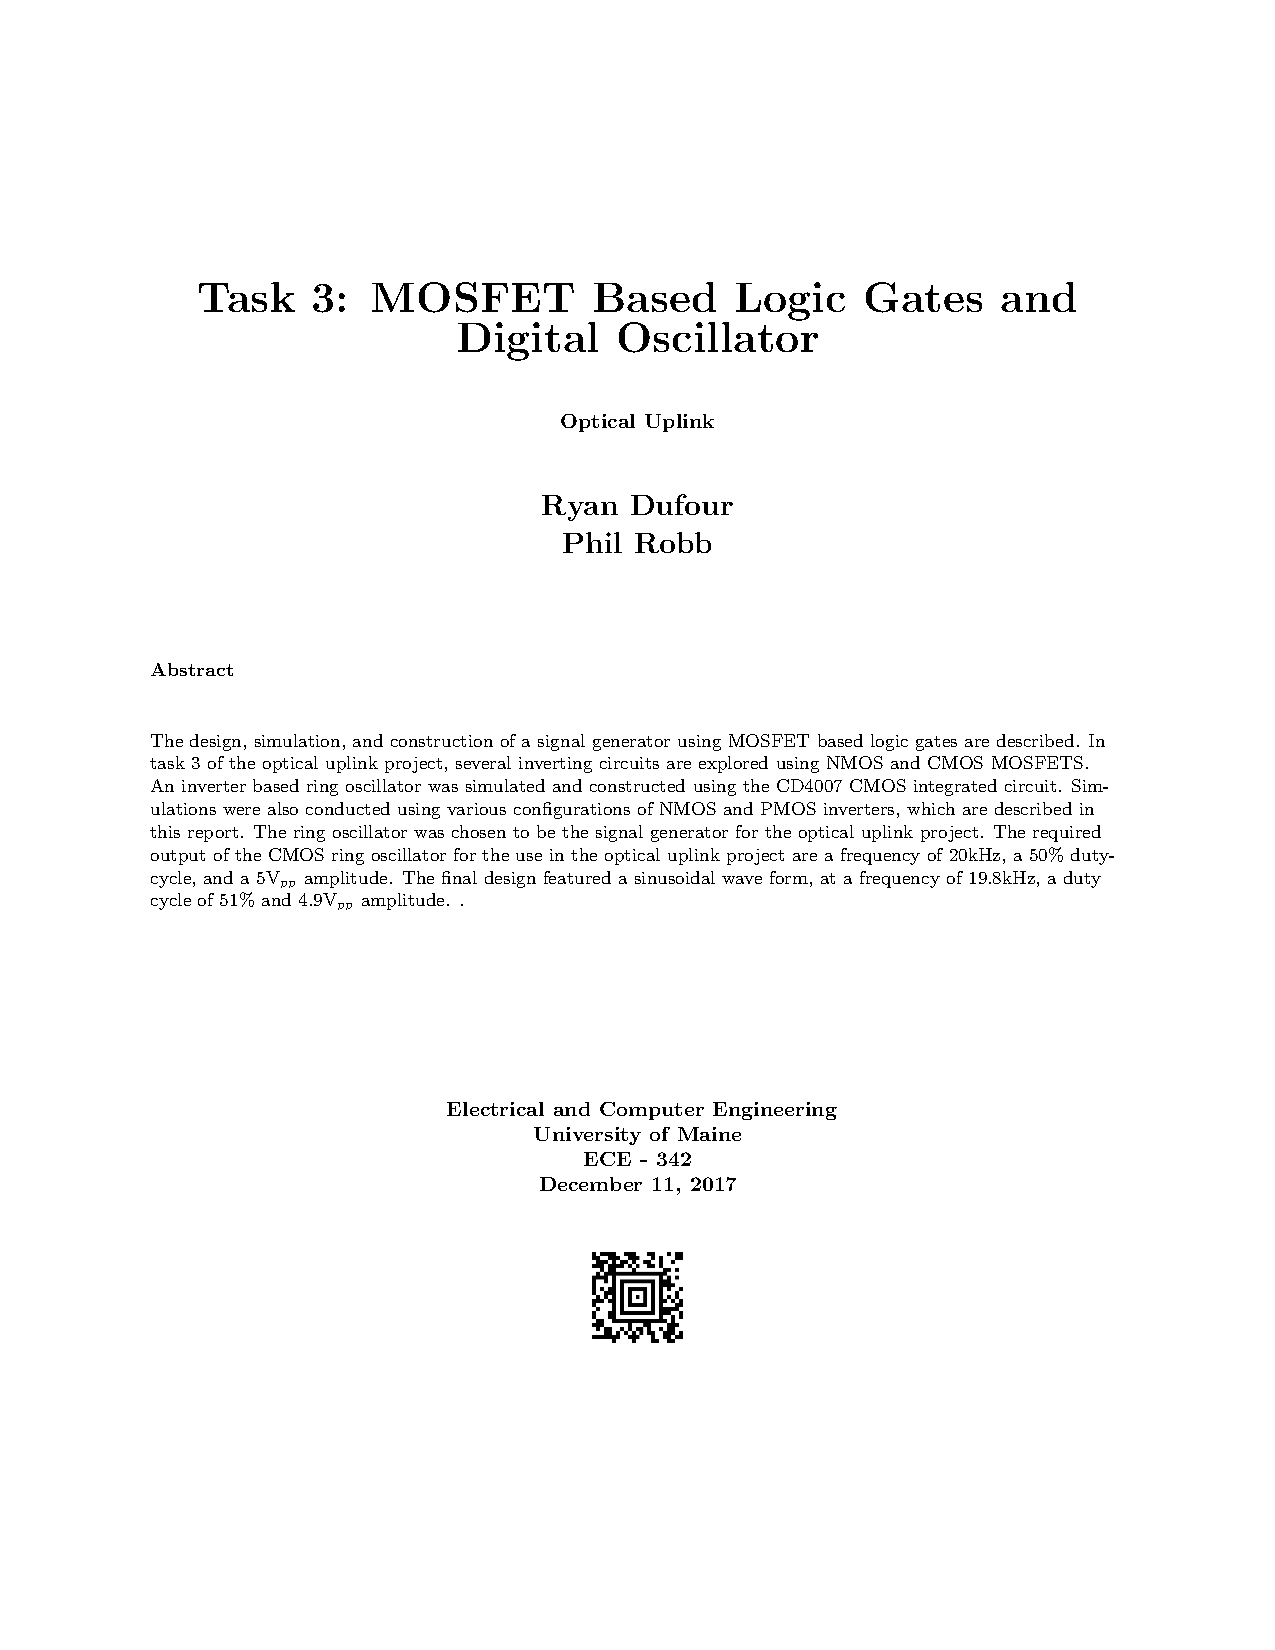
\includepdf[pages={-}]{Lab_3.pdf}

\section{LED Driver}
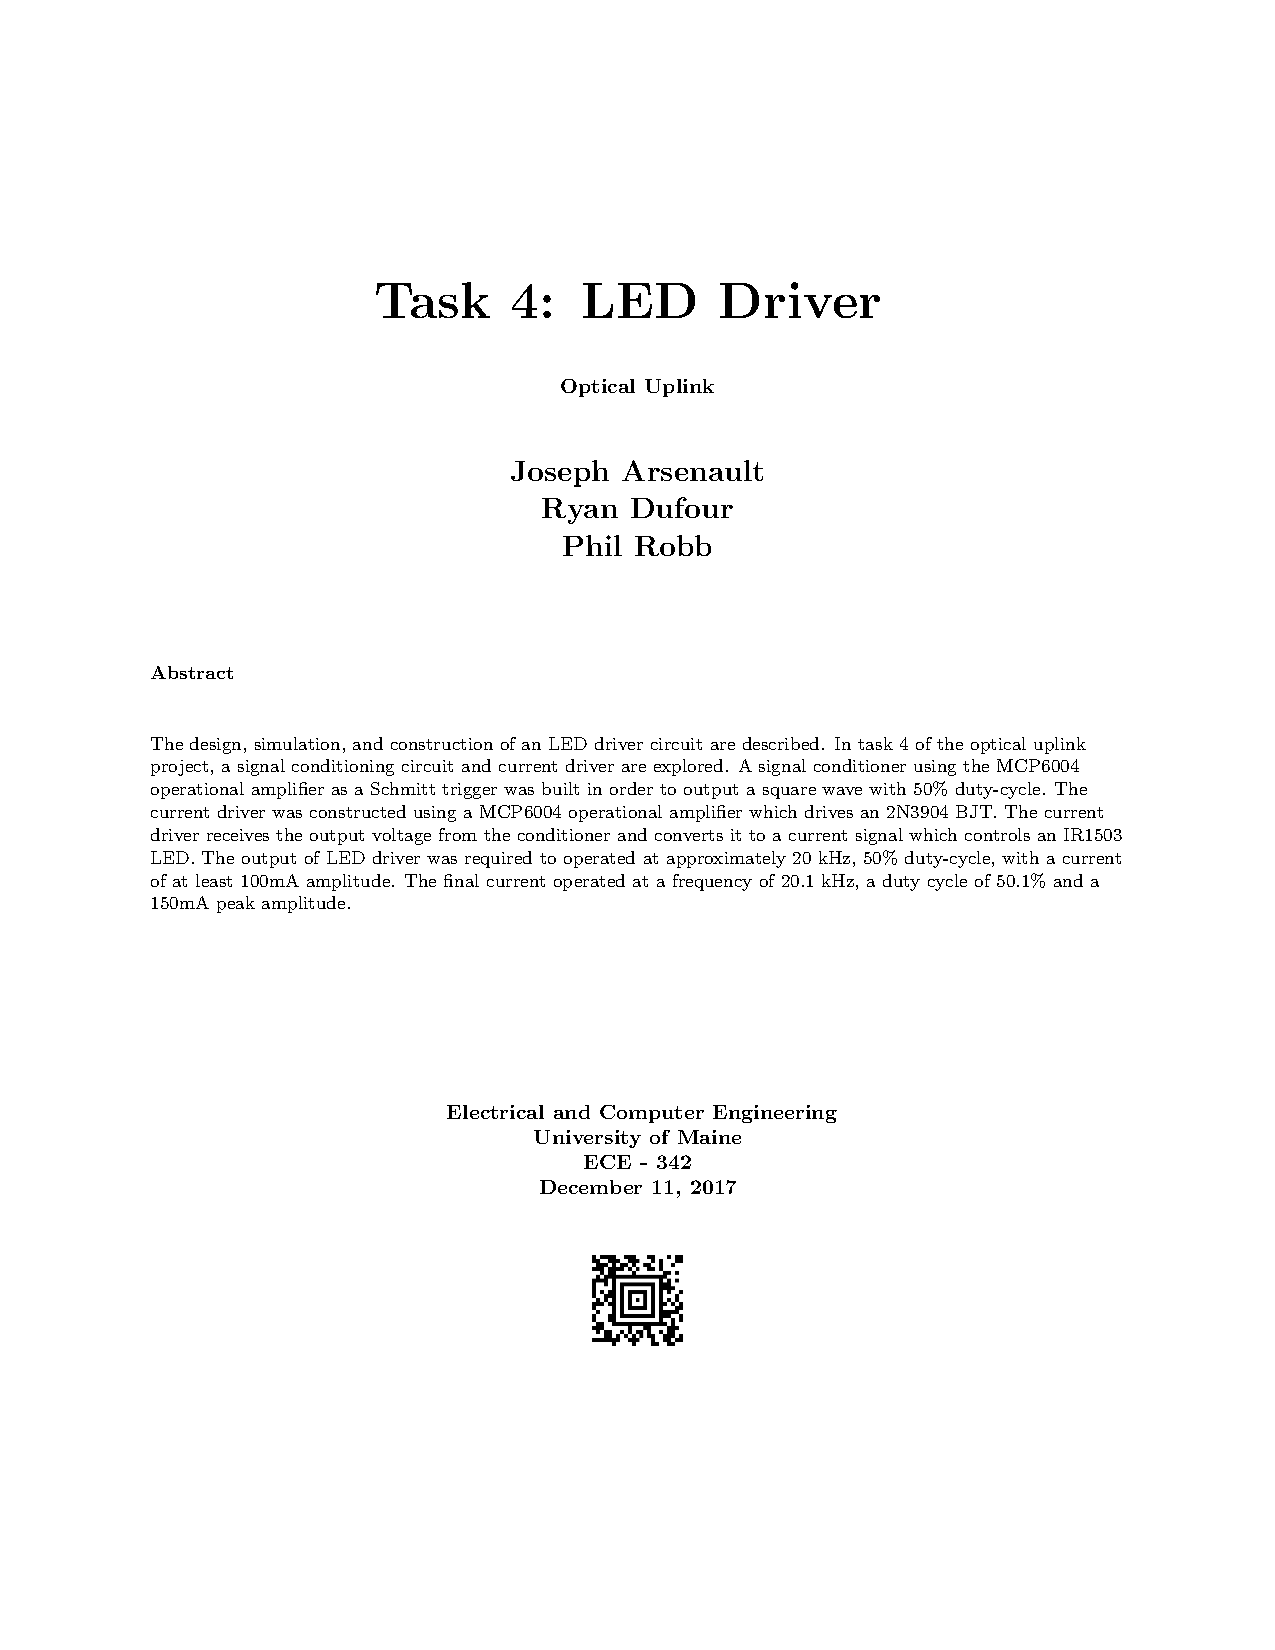
\includepdf[pages={-}]{Lab_4.pdf}	

\section{Voltage Amplifier}
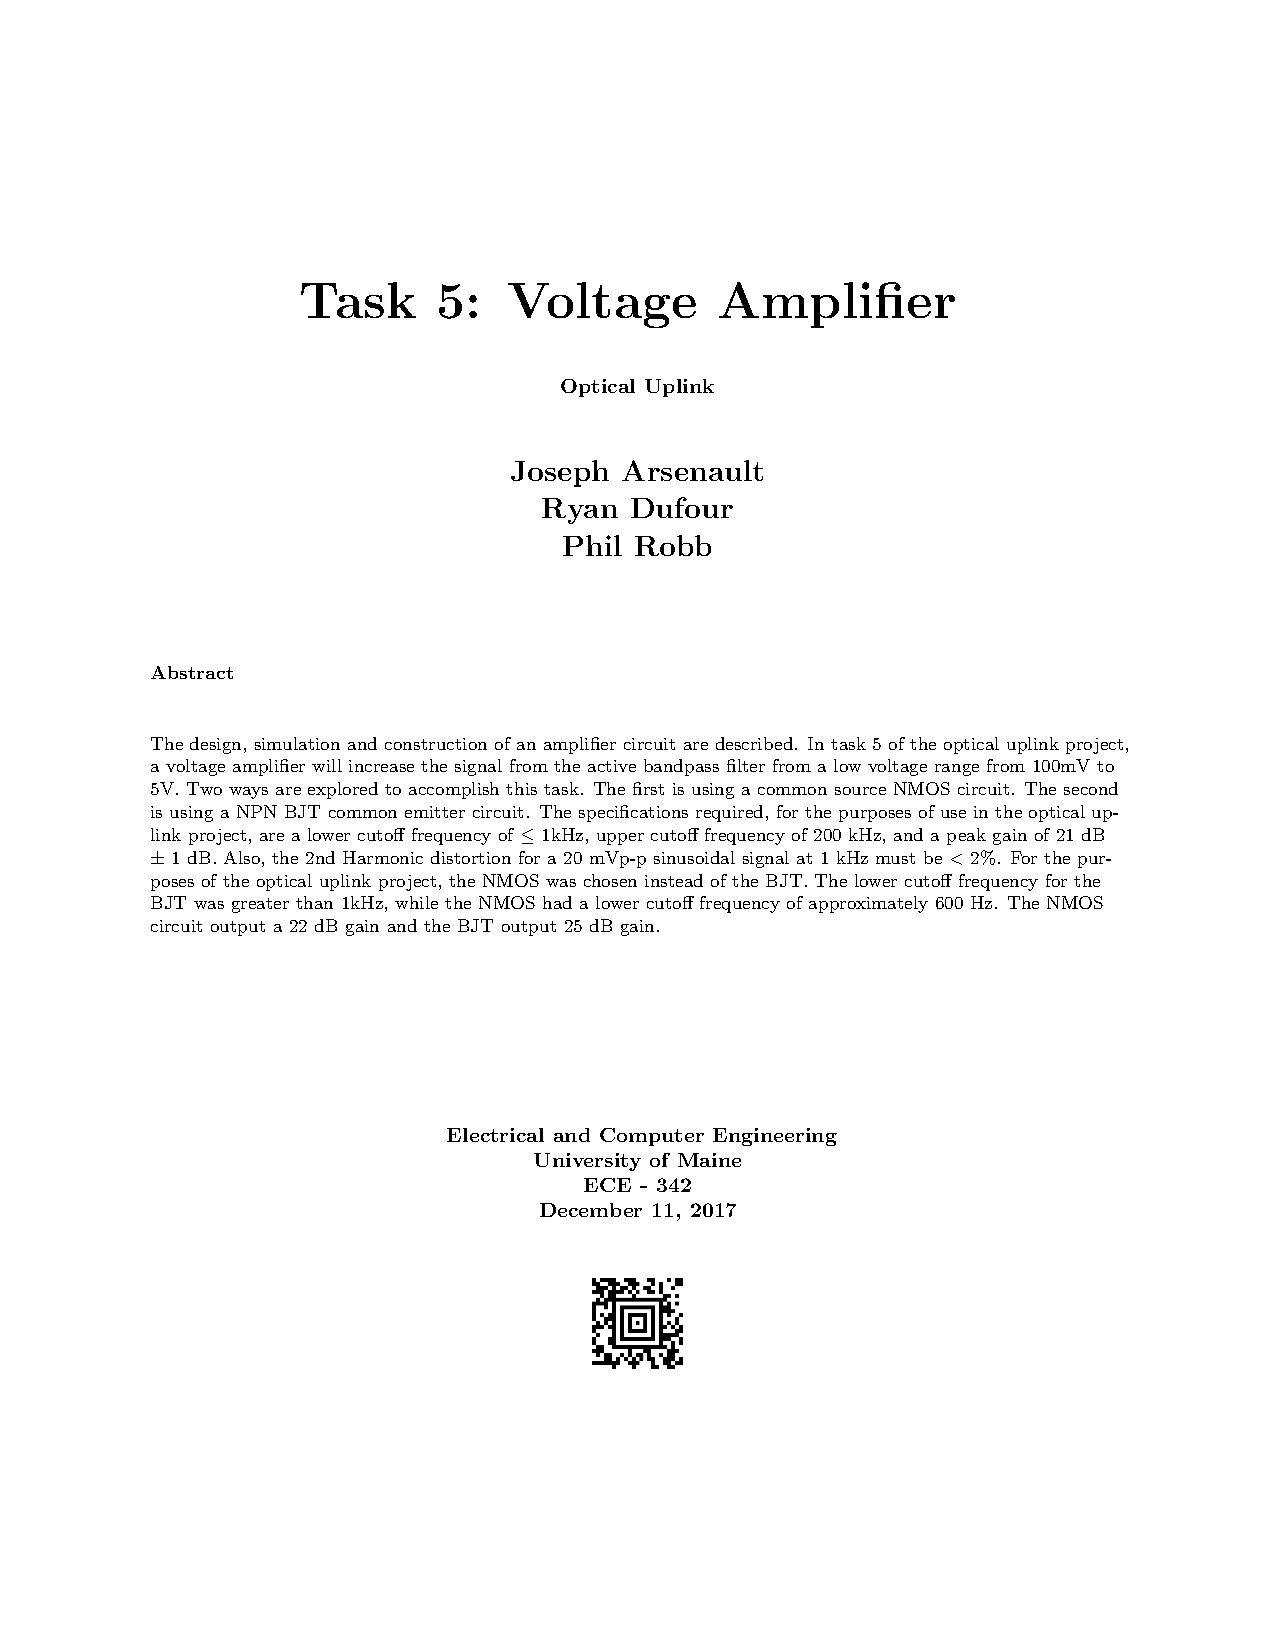
\includepdf[pages={-}]{Lab_5.pdf}		



\end{appendices}




\begin{comment}
\section{References}

\noindent [1] N.W. Emanatoglu.(2017) Lab $\#1$; photodetector and transimpedence amplifier [Online]. Available: http://web.eece.maine.edu/~kotecki/ECE342/labs/ECE342_2017_Lab2.pdf
\newline

\noindent [2] D.E. Kotecki Lab.(2017) Resistively Loaded MOSFET Gate [Online]. Available: http://web.eece.maine.edu/~kotecki/ECE342/labs/ECE342_2017_Lab3_Inverter.pdf
\newline

\noindent [3] N.W. Emanatoglu.(2017) Lab $\#1$; photodetector and transimpedence amplifier [Online]. Available: http://web.eece.maine.edu/~kotecki/ECE342/labs/ECE342_2017_Lab2_MFBF.pdf
\newline

\noindent [4] Cree.(2014) 5-mm Blue and Green LED [Online]. Available http://www.cree.com/led-components/media/documents/C503B-BAS-BAN-BCS-BCN-GAS-GAN-GCS-GCN-1094.pdf
\newline

\noindent [5] Kingbright.(2017) WP7113SGC [Online]. Available: http://www.us.kingbright.com/images/catalog/SPEC/WP7113SGC.pdf
\newline

\noindent [6] D.E. Kotecki Lab.(2017) PIN Silicon Photodiode [Online]. Available: http://web.eece.maine.edu/~kotecki/ECE342/datasheets/OP993-999\_0.pdf
\newline

\noindent [7] Kingbright.(2017) WP7113SEC/J3 [Online]Available: http://www.kingbrightusa.com/images/catalog/SPEC/WP7113SEC-J3.pdf
\newline

\noindent [8] Everlight.(2006) IR1503 [Online]. Available: https://radiodetali.com/media/catalog/product/i/r/ir1503.pdf
\newline
\end{comment}

\end{document}
